\documentclass{article}
	% This is where you include the preambles for every file.
\usepackage{amssymb}
\usepackage{amsmath}
\usepackage{mathtools}
\usepackage{csvsimple}
\usepackage{graphicx}
\usepackage{placeins}
\usepackage{siunitx}
\usepackage{spreadtab}
\usepackage[euler]{textgreek}
\usepackage{url}
\usepackage{geometry}
\usepackage{listings}
\geometry{left=20mm}

\begin{document}
	\begin{titlepage}
		\centering
		\Huge{Experiment 3} \\
		\huge{Characterization of Semiconductors} \\
		\vspace{1cm}
		\large{EECS 170A - Lab Bench \#1} \\
		\large{\today} \\
		\vspace{1cm}
		\normalsize{Roman Parise (59611417)} \\
		\normalsize{Krishan Solanki (38154673)} \\
		\normalsize{Jason Wang (42873192)} \\
	\end{titlepage}
	% This is where the body of each file goes
	\section{Procedure}
The objective of this lab is to observe basic semiconductor characteristics of a wafer after a hot-probe is placed on it. The hot probe helps determine if the semiconductor is n-type or p-type. The resistivity is also measured using a four-point probe. The experiment begins by heating up a soldering iron and then placing it on a silicon wafer. Two probes are placed on the wafer, one near the soldering iron and the other far away. The voltage between the hot and cold probes is then measured. After completing the first part with the soldering iron, the final part deals with measuring the resistivity after a four-point probe is placed on the silicon wafer. \\

	\section{Results and Analysis}
	\subsection{Hot Probe Technique}
	The hot probe technique is utilized to determine the type of unknown semiconductor material, pieces of silicon wafer. The first wafer tested is a large piece of silicon wafer approximately one centimeter in width and three centimeters in length. The specific piece of silicon wafer tested is shown in the image below:

	\FloatBarrier
	
	\begin{figure}[h!]
		\centering
		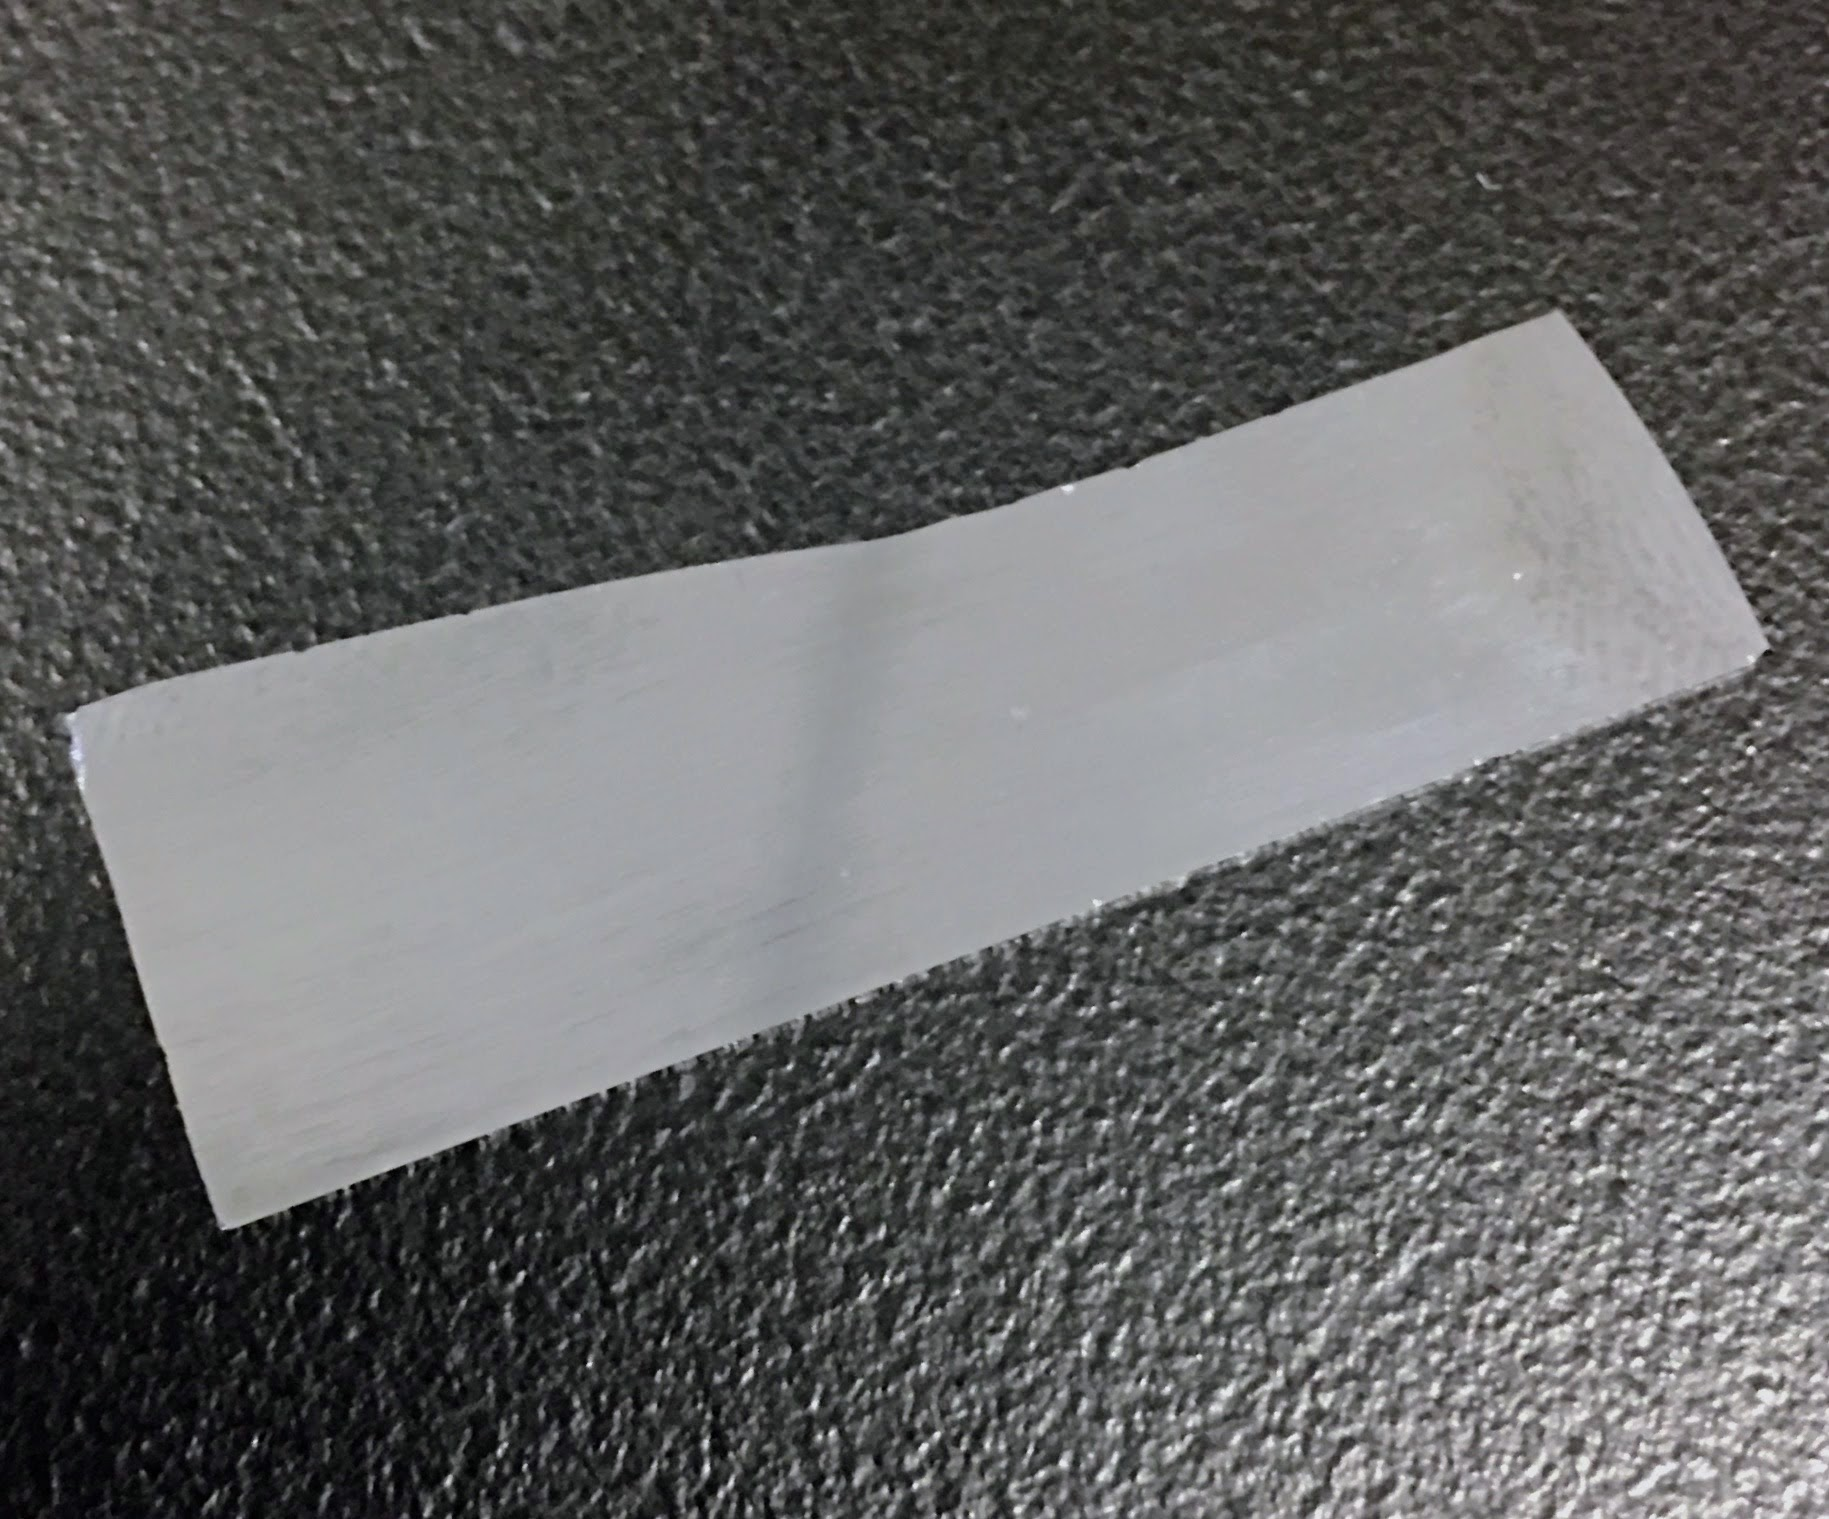
\includegraphics[scale=0.1]{../images/wafer.JPG}
		\caption{Image of First Silicon Wafer Tested with Hot Probe Technique}
		\label{fig:wafer}
	\end{figure}

	\FloatBarrier
	
	In the hot probe technique, a temperature gradient is introduced to the silicon wafer through contact with a hot probe, in this case a soldering iron, to one end of the wafer. Then, a digital voltmeter with high impedance is used to measure the voltage across the wafer from the hot end to the cool end (positive terminal to the hot end, negative terminal to the cool end). The sign of the voltage indicates the type of the semiconductor material. The circuit schematic below portrays the setup of the hot probe technique:

	\FloatBarrier
	
	\begin{figure}[h!]
		\centering
		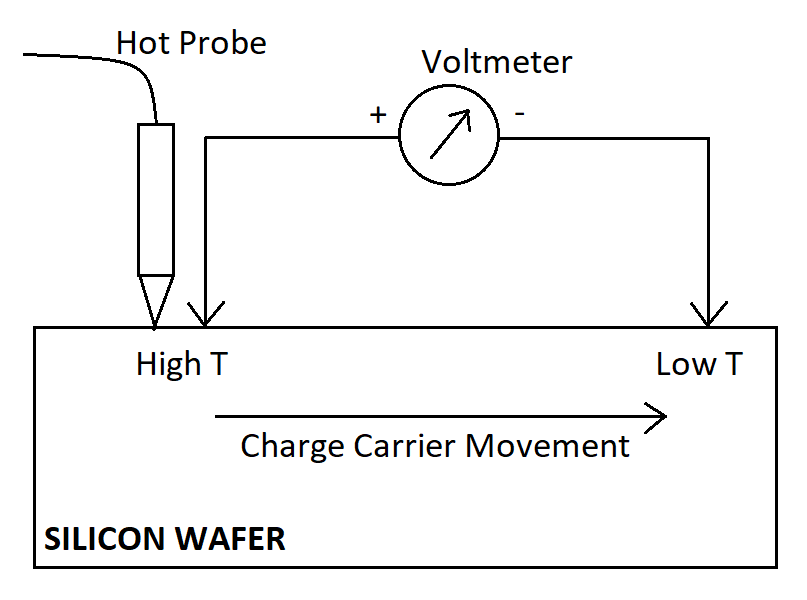
\includegraphics[scale=0.7]{../images/hot_probe_schematic.PNG}
		\caption{Circuit Schematic of Hot Probe Technique}
		\label{fig:hot_probe_schematic}
	\end{figure}

	\FloatBarrier
	
	The hot probe and positive terminal of the digital voltmeter is first introduced to one end of the silicon wafer and is set there for approximately 30 seconds to generate the temperature gradient across the wafer. Then, the negative terminal of the voltmeter, cool due to no prior contact with the heated wafer and hot probe is introduced to the other end of the wafer. With the increased temperature difference between both ends of the wafer as a result of this method, a more optimal voltage measurement can be achieved.
	
	The following voltages are indicated by the digital voltmeter with $\pm 1 V$ fluctuations in each case:
	
	\FloatBarrier

	\begin{table}[h!]
		\centering
		\caption{Hot Probe Measurements for First Wafer}
		\label{tab:hot_probe_measurements_p_type}
		\csvautotabular{../tables/hot_probe_measurements_p_type.csv}
	\end{table}

	\FloatBarrier
	
	The high negative voltages in Table \ref{tab:hot_probe_measurements_p_type} clearly indicate that the first wafer tested is a p-type semiconductor. This is because the temperature gradient causes charge carriers to move towards the cooler side of the wafer, thus inducing a current in the material and ultimately a voltage difference across the semiconductor. If the semiconductor material is p-type, then the charge carriers, holes, will migrate from the hot end to the cool end, leaving ionized acceptors with negative charge at the hot end. This polarizes the material so that the hot end is negatively charged and the cool end is positively charged. Measuring voltage from the hot end to the cool end in this case would then yield a negative result. For n-type semiconductors, the charge carriers, electrons, also migrate from the hot end to cool end, which then leaves ionized donors with positive charge at the hot end. This polarizes the material so that the hot end is positively charged and the cool end is negatively charged. Measuring voltage from the hot end to the cool end in this case would then yield a positive result.
	
	During testing of n-type silicon wafers, voltage measurements across the ends of the wafers were very noisy. Below are the measurements taken for two n-type wafers:
	
	\FloatBarrier

	\begin{table}[h!]
		\centering
		\caption{Hot Probe Measurements for N-type Wafers}
		\label{tab:hot_probe_measurements_n_type}
		\csvautotabular{../tables/hot_probe_measurements_n_type.csv}
	\end{table}

	\FloatBarrier
	
	\subsection{Four-Point Probe Method}

\FloatBarrier

\begin{figure}[h!]
	\centering
	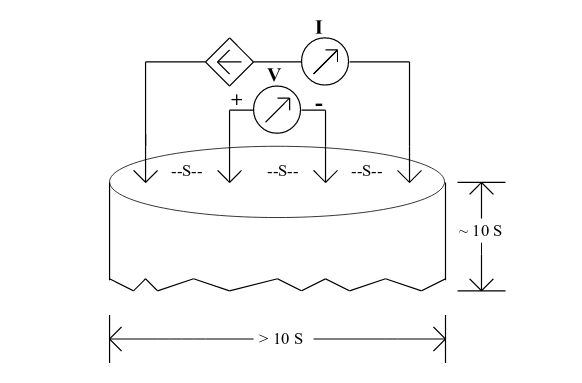
\includegraphics[scale=0.5]{../images/three_pt_probe.PNG}
	\caption{Four-Point Probe Setup}
	\label{fig:four_pt_setup}
\end{figure}
{\footnotesize Source: Lab manual}

\FloatBarrier
% Derive the sheet resistance equation
% TODO Pic of wafer
Let $t$ be the thickness of the wafer and $\rho$ be its resistivity. The sheet resistance $R_s$ is defined to be:

\begin{equation}
\label{eq:rs_def}
R_s = \frac{ \rho }{ t }
\end{equation}

When the current source delivers current to the silicon wafer, the current moves uniformly near the surface due to the negligible thickness of the wafer. Thus, the current spreads normal to the face of a cylinder around the center where the probe lies. A similar phenomenon occurs at the other probe of the current source, but the current moves toward rather than away from the probe.
The voltage is measured with different probes, each a distance $s$ away from the respective probes measuring current. The current from each current probe passes between the voltage probes. Thus, a resistance $R$ between the two voltage probes can be defined.
Let $L$ be the length of a slab along which current travels, and $A$ be its cross-sectional area. Resistance can then be defined as:

\begin{equation}
\label{eq:resistance_def}
R = \frac{ \rho L }{ A }
\end{equation}

At a radius $r$ from the location of a current source probe, current can be modeled as flowing through a cylindrical surface of height $t$ and radius $r$. This is due to the circular spread of current from the current source probe. The effective "area" through which current flows is thus a function of $r$:

\begin{equation}
\label{eq:area_fn}
A(r) = 2 \pi r t
\end{equation}

The first voltage probe occurs at a distance $s$ from the current probe. The current then flows $s$ further to reach the other voltage probe. Thus, $r$ varies from $s$ to $2s$. Clearly, equation \ref{eq:resistance_def} is difficult to apply since $A$ is a function of $L$ in the experiment. The longer $L$, or $r$ in this particular case, the larger $A$ becomes.
For a small distance around a particular value of $r$, $A$ is effectively constant. The interval $[0,r]$ can be partitioned into small segments of length $\Delta r$ with an essentially constant resistance for that particular segment. Since these small resistances would all be in series, the equivalent resistance is simply their sum. The approximation becomes better with smaller values of $\Delta r$:

\begin{equation}
\label{eq:res_btwn_probes}
\begin{aligned}
R = \lim_{n\to\infty} [ \frac{ \rho \Delta r }{ A(s) } + \frac{ \rho \Delta r }{ A(s + \Delta r) } + ... + \frac{ \rho \Delta r }{ A(s + n \Delta r = 2s ) } ] \\
= \lim_{n\to\infty} \sum_{i=0}^{n} \frac{ \rho \Delta r }{ A( s + i\Delta r )} \\
= \int_{s}^{2s} \frac{ \rho dr }{ A(r) } \\
= \int_{s}^{2s} \frac{ \rho dr }{ 2 \pi r t } \ ( \ substitute \ equation \ (\ref{eq:area_fn}) \ ) \\
= \frac{ \rho }{ 2 \pi t } \int_{s}^{2s} \frac{ dr }{ r } \\
= \frac{ \rho }{ 2 \pi t } ln(2)
\end{aligned}
\end{equation}

The resistance is more traditionally defined as the ratio between the voltage over a circuit element to the current through the circuit element. The voltage is measured to be $V$. The current from one probe is $I$, and the current from the other probe is $-I$. They overlap in the region between the voltage probes, and the effective current becomes $2I$:

\begin{equation}
\label{eq:alt_res_btwn_probes}
R = \frac{V}{2I}
\end{equation}

Equating (\ref{eq:res_btwn_probes}) and (\ref{eq:alt_res_btwn_probes}) and letting $F = \frac{\pi}{ln(2)}$, known as the correction factor, the following result is obtained:

\begin{equation}
\label{eq:sheet_res_vi}
R_s = \frac{\rho}{t} = \frac{ FV }{ I }
\end{equation}

If the sheet resistance is acquired, then $\rho$ can be ascertained by simply multiplying $R_s \cdot t$.

% V,I data table with Rs and rho calculations

\FloatBarrier

\begin{table}[h!]
	\centering
	\caption{Four-Point Probe Measurements}
	\label{tab:fpp_measure}
	\csvautotabular{../tables/data_table_4ptprobe.csv}
\end{table}

\FloatBarrier

\begin{table}[h!]
	\centering
	\caption{Four-Point Probe Results}
	\label{tab:fpp_results}
	\csvautotabular{../tables/results_table_4ptprobe.csv}
\end{table}

\FloatBarrier

\FloatBarrier

\begin{figure}[h!]
	\centering
	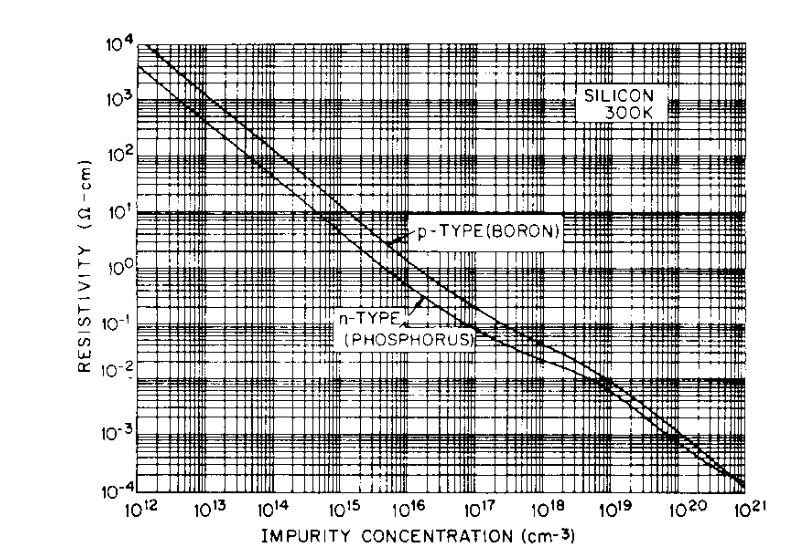
\includegraphics[scale=0.5]{../images/resistivity_graph.PNG}
	\caption{Resistivity vs Impurity Concentration in Silicon}
	\label{fig:res_vs_imp}
\end{figure}
{\footnotesize Source: Lab manual}

\FloatBarrier

% Find impurity concentration
Given the resistivity in table (\ref{tab:fpp_results}), the impurity concentration is approximately $2 \times 10^{17} [\frac{donors}{cm^3}]$. The wafer given is n-type, so the impurity present would be donors, which is typically an element like phosphorus or arsenic [lab manual].

Note that the theory above can be applied since $d >> s$ (by a factor of about 10), and the thickness of the wafer $t$ is also much less than $s$ and $d$ by about three orders of magnitude. The thickness of the wafer is crucial because the above analysis assumes that the current largely travels in an outward cylindrical fashion rather than spherically. If the wafer were thick, then a considerable portion of the current would travel through the interior of the wafer, making the analysis require a spherical current rather than the cylindrical current considered. Moreover, if $d >> s$ were to fail, then as the current spreads cylindrically from the current probe, it would be limited in its spread by the dimensions of the wafer. So, the integration to find the resistance would be tricky to perform. $F$ ends up being smaller in these cases [\ref{itm:resistivity_simplification}]. % TODO Proper citation

% TODO Resistivity graph and cite lab manual

% Linear regression explanation

The resistance is estimated from one value of current and voltage. However, this is not the most reliable way of performing resistance measurements. The issue is individual resistance measurements can be subject to experimental errors and nonlinear variations in the device.
Ideally, there would be a method of capturing and averaging out various measurements of resistance along an IV-curve, while still keeping a simple linear model. The best way of doing this is linear regression. Without going into a derivation and the technical details underlying the theory of linear regression, the idea is to find the best linear relationship between two variables, current and voltage in this case:

\begin{equation}
\label{eq:linear_reg}
V = RI + b
\end{equation}

Then, take multiple $(I,V)$ measurements in the lab, and find the values of $R$ and $b$ that produce a line that most "closely" fits the data points. "Most closely" essentially means the values of $R$ and $b$ that minimize the squared error between the best fit line and the measured data points [\ref{itm:best_fit_line}].
The slope $R$ in this line would simply be the resistance, or more specifically $\frac{V}{I}$ in the lab. $R_{s}$ can then be acquired using equation (\ref{eq:sheet_res_vi}). This model takes into account various other $(I,V)$ points, but still maintains the linear simplicity of the static resistance model.

	
	\section{Discussion}
	\subsection{Hot Probe Technique}
	While the hot probe technique yielded good results for the p-type silicon wafer, it did not produce discernible results for the n-type silicon wafers. This may be due to the size of the p-type silicon wafers that are tested. The areas of the n-type wafers that were subject to the hot probe technique are approximately one cubic centimeter. Due to the small size of the wafers, the contact with the hot probe may have caused uniform heating in the wafers rather than the desired temperature gradient. This then causes the wafer to essentially be at thermal equilibrium, thus no polarizing effect occurs and no significant voltage can be measured. Also, the higher mobility of electrons as charge carriers over holes may have played a role in the high fluctuation of the p-type semiconductors tested. Because of the free electrons' higher tendency to move in the material, the stability of the voltage measured across the ends of the p-type wafers may have suffered as a result. The hot probe technique in this experiment seems to be imprecise and crude in nature due to the instruments used and wafers tested. However, because the purpose of the experiment is not precision measurements but rather determination of type for semiconductor materials, the set up is adequate for that purpose.

	\subsection{Four-Point Probe Method}
The measured resistivity is on the order of $10^{-2}$, quite a small resistivity. The theory used to calculate the resistivity is valid because the distances between probes is negligible in comparison to the dimensions of the wafer and the wafer is extremely thin in comparison to the other measured lengths. Using this resistivity value, the impurity concentration is determined to be quite high, around $2 \times 10^{17} [\frac{donors}{cm^3}]$. The high impurity concentration explains why the resistivity is so low. When a large number of donors are present in silicon, more carrier electrons are generated in the conduction band. Thus, for the same potential difference, more charges can move around, and thus a higher current is possible. Therefore, the resistivity is expected to be low. However, a more thorough analysis is required before the impurity concentration figure is finalized. More data points and a linear regression analysis is required to determine a more accurate value for the resistivity and therefore the carrier concentration.

	\section{References}
	\begin{enumerate}
		\item \label{itm:resistivity_simplification} \url{http://astro1.panet.utoledo.edu/~relling2/teach/archives/4580.6280.2011/20111025_lecture_4.2_phys4580.6280.pdf}
		\item \label{itm:electromagnetic_compatibility} \url{https://books.google.com/books?id=nZzOAsroBIEC&pg=SA13-PA52&lpg=SA13-PA52&dq=electromagnetic+compatibility+handbook+static+vs+dynamic+resistance&source=bl&ots=bB_L6xJM1S&sig=zkE0IWOaOjY7DQSPjdWZzDDJID4&hl=en&sa=X&ved=0ahUKEwj0h-DGgJfXAhVR3GMKHa9ODXEQ6AEIKDAA#v=onepage&q=electromagnetic\%20compatibility\%20handbook\%20static\%20vs\%20dynamic\%20resistance&f=false}
		\item \label{itm:best_fit_line} \url{http://www.mit.edu/~6.s085/notes/lecture3.pdf}
	\end{enumerate}

\end{document}
